%=======================================================
%	PACKAGES AND THEMES
%=======================================================
\documentclass[8pt]{beamer}
\mode<presentation> {
\usepackage{etex}
\usetheme{Boadilla}
\definecolor{navyblue}{rgb}{0.0, 0.0, 0.5}
\definecolor{dkgreen}{rgb}{0,0.6,0}
\definecolor{gray}{RGB}{64, 64, 64}
\definecolor{teal}{RGB}{0, 102, 102}
\definecolor{mauve}{rgb}{0.58,0,0.82}
\usecolortheme[named = navyblue]{structure}
\setbeamercolor{normal text}{fg = gray}
\setbeamercolor{frametitle}{fg = white, bg = navyblue}
\setbeamerfont{framesubtitle}{size = \normalsize}
\setbeamerfont{caption}{size=\footnotesize}
\setbeamercolor{page number in head/foot}{fg = gray}
\setbeamertemplate{footline}%[frame number]
}


\usepackage{graphicx} % Allows including images
\usepackage{booktabs} % Allows the use of \toprule, \midrule and \bottomrule in tables
\usepackage{multicol}
\usepackage[export]{adjustbox}
\usepackage{colortbl}
\usepackage{graphicx} 

\usepackage{tikz}
\usepackage{fancybox}
\usepackage[absolute, overlay]{textpos}
\usepackage{multirow}
\usepackage{siunitx}
\usepackage{tcolorbox}


\usepackage{tikz}
\usepackage{calc}
\newlength{\outerradius}
\newlength{\innerradius}
\setlength{\outerradius}{0.50cm}
\setlength{\innerradius}{0.35cm}

%Damit wir Quellcode nutzen können.
\usepackage{listings}
\lstset{numbers=left,
	numberstyle=\tiny,
	numbersep=5pt,
	breaklines=true,
	showstringspaces=false,
	frame=l ,
	xleftmargin=15pt,
	xrightmargin=15pt,
	basicstyle=\ttfamily\scriptsize,
	stepnumber=1,
	keywordstyle=\color{blue},          % keyword style
  	commentstyle=\color{dkgreen},       % comment style
  	stringstyle=\color{mauve}         % string literal style
}
%Sprache Festelegen
\lstset{language=R}


%=======================================================
%	TITLE PAGE
%=======================================================

\title{\textbf{Descriptive Network Analysis B}\\
	      {\color{teal}{--Seminar--}}}

\author{Yasemin Aslan}

\institute
{
SPRU (Science Policy Research Unit) \\
Business School\\
University of Sussex \\

\medskip

\medskip

\medskip

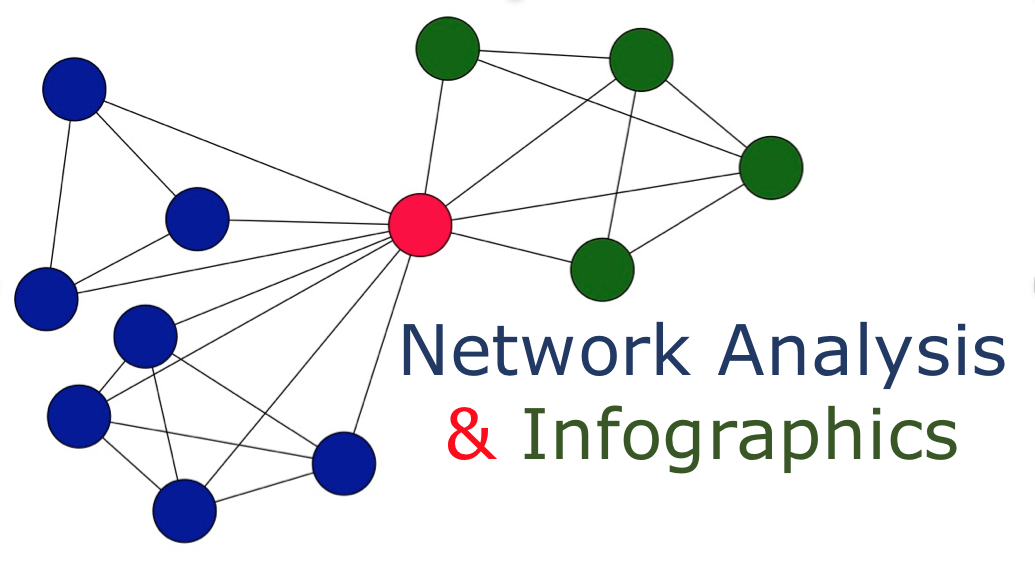
\includegraphics[width=2.5cm]{../_shared_pics/logo}

\medskip

\textit{{\color{dkgreen}{Week 5: 25 February 2022}}}\\
}


\date{} % Date, can be changed to a custom date

\begin{document}

\begin{frame}
\titlepage % Print the title page as the first slide

\begin{textblock*}{10pt}(0pt, 0.9\textheight)

\includegraphics[width=4cm]{../_shared_pics/SPRU.png}
\end{textblock*}

\end{frame}



%=======================================================
%	Learning outcomes
%=======================================================


\begin{frame}
\frametitle{\insertsection}
\framesubtitle{Learning Outcomes}

\centering
\begin{tabular}{lp{5.5cm}l}
\toprule
\multicolumn{2}{l}{\textbf{Learning outcome}} & \textbf{Assessment mode}\\
\hline
\\
1 & 
Explain the concept of network and list the main network indicators & 
ESS\\
\\
2 &  
Describe and apply the major techniques for the collection of network data and their statistical analysis & 
ESS, GPN + GWS\\
\\
\rowcolor{green!20}3 & 
Identify the main characteristics of networks by means of network measures  & 
ESS, GPN + GWS\\
\\
4 &
Employ network analysis techniques to produce network data-based infographics & 
GPN + GWS\\
\\
\bottomrule
\multicolumn{3}{l}{\scriptsize Note: ESS: Essay; GPN: Group Presentation; GWS: Group Written Submission}\\
\end{tabular}

\end{frame}

%------------------------------------------------



%=======================================================
%	Intro slides
%=======================================================

\begin{frame}
\frametitle{Overview}
\tableofcontents[hideallsubsections]
\end{frame}



%=======================================================
% Centrality measures [recap]
%=======================================================
\section{Centrality measures [recap]}
%------------------------------------------------

\bgroup
\setbeamercolor{background canvas}{bg = navyblue}
\begin{frame}[plain]{}
\begin{center}
\color{white}{\Huge\insertsection}
\end{center}
\end{frame}
\egroup

%------------------------------------------------

\begin{frame}
\frametitle{\insertsection}
\framesubtitle{\insertsubsection}

\small
\begin{table}
\begin{tabular}{p{3cm}p{7.5cm}}
\toprule
\textbf{Centrality measure} 	&	\textbf{Interpretation} \\
\hline
\\
Degree 		&	How many nodes can a node reach directly?\\
			&	\textit{\color{blue}information flow, popularity, influence}\\
\\
Closeness        &	    How fast can a node reach every node in the network?\\
			&	\textit{\color{blue}speed, diffusion, efficiency}\\
\\
Betweenness        &	How likely is a node to be part of the most direct route between two nodes in the network?\\
			&	\textit{\color{blue}control, fragmentation, brokerage}\\
\\
Bonacich's centrality 	&	How well is an actor connected to other well-connected actors in the network?\\ 
			&	\textit{\color{blue}power, comprehensive view of the network}\\
\\
Weighted centrality     & Use of the information about the strength of the ties (and distribution of these in the case of Opsahl's centrality)\\
\bottomrule
\end{tabular}
\end{table}
\end{frame}

%------------------------------------------------ 




%=======================================================
% Centrality measures in igraph
%=======================================================
\section{Centrality measures in \textit{igraph}}
%------------------------------------------------

\bgroup
\setbeamercolor{background canvas}{bg = navyblue}
\begin{frame}[plain]{}
\begin{center}
\color{white}{\Huge\insertsection}
\end{center}
\end{frame}
\egroup

%------------------------------------------------

\begin{frame}
\frametitle{\insertsection}

Your source of all igraph functions: \url{http://igraph.org/r/doc/}

\end{frame}

%------------------------------------------------

\begin{frame}
\frametitle{\insertsection}

\small
\begin{table}
\begin{tabular}{ll}
\toprule
\textbf{Measure}        		& \textbf{igraph function} \\
\hline
\\
Degree                  		& \textbf{degree(...)}\\
\\
Closeness               		& \textbf{closeness(...)}\\
\\
Betweenness             		& \textbf{betweenness(...)}\\
\\
Centralization					& \textbf{centr\_degree(...)}\\
								& \textbf{centr\_clo(...)}\\ 
								&  \textbf{centr\_betw(...)}\\
\\
Bonacich's centrality			&  \textbf{power\_centrality(...)}\\
								& (see section other scripts for calculation)\\
\\
Weighted degree					& \textbf{strength(...)}\\
Weighted closeness				& \textbf{closeness(...)}\\
Weighted betweenness 			& \textbf{betweenness(...)}\\
\\
Opsahl' weighted centralities	& \textbf{degree\_w(...)}\\
								& \textbf{closeness\_w(...)}\\
								&\textbf{betweenness\_w(...)}\\
								&from the \textbf{tnet} package\\
								&(see section other scripts for calculation)\\
\bottomrule 
\end{tabular}
\end{table}
\end{frame}


%------------------------------------------------

%%=======================================================
%	Group Exercise
%%=======================================================
\section*{Group Exercise}

%------------------------------------------------

\bgroup
\setbeamercolor{background canvas}{bg = navyblue}
\begin{frame}[plain]{}
\begin{center}
\color{white}{\Huge\insertsection}
\end{center}
\end{frame}
\egroup

%------------------------------------------------

%------------------------------------------------

\begin{frame}
\frametitle{\insertsection}

\begin{itemize}

\item {Creating network(s) by using real data}
	\begin{itemize}
	\item Create at least one network
	\item Apply related network/node level measures
	\item Interpret the results in a comparative/complementary way
	\end{itemize}

\medskip

\item {UKRI-MRC Research Grants Data for the year 2006-2020}
	\begin{itemize}
	\item 250 projects as a sample
	\item Use full data to create your network(s) or create a subgraph(s)
       \item Use country, sector, year, expenditure variables as attributes to complement your analysis
	\end{itemize}

\medskip

\item {Randomly selected groups}

\medskip

\item {Coming weeks...}
	\begin{itemize}
	\item Apply the metrics/concepts that we will learn weekly
	\item Each group will make a short presentation
	\end{itemize}


		
\end{itemize}

\end{frame}

%------------------------------------------------


%%=======================================================
%	Next time ...
%%=======================================================
\section*{Next time ...}

%------------------------------------------------

\bgroup
\setbeamercolor{background canvas}{bg = navyblue}
\begin{frame}[plain]{}
\begin{center}
\color{white}{\Huge\insertsection}
\end{center}
\end{frame}
\egroup

%------------------------------------------------

\begin{frame}
\frametitle{\insertsection}

\begin{itemize}

\item 	\textbf{Lecture: Descriptive network analysis C}
	\begin{itemize}
	\item Node-level measures (brokerage measures)
	\end{itemize}

\medskip
\medskip


\item 	\textbf{Seminar: Descriptive network analysis C}
	\begin{itemize}
	\item Assessment of node-level measures (brokerage measures)
	\end{itemize}
	

		
\end{itemize}

\end{frame}

%------------------------------------------------






\end{document}